\begin{figure}[h]
  \centering
  
%segundo bloco de figuras
  \begin{tabular}{@{}c@{} p{1.5cm} @{}c@{} }
   \centering 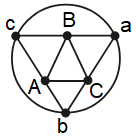
\includegraphics[width=2.5cm]{./img/octaedro.png} & &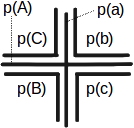
\includegraphics[width=2.9cm]{./img/representacaoOctaedro.png}  \\[\abovecaptionskip]
    \footnotesize \centering (a) The octahedral $O_3$ graph  & &  \footnotesize(b) $B_1$-EPG representation of the graph $O_3$
  \end{tabular}

 \caption{The octahedral $O_3$ graph and its  $B_1$-EPG representation}\label{fig:octaedro}
\end{figure}